\chapter{The Small Leaved Shrub Problem}

If the profusion of vines and epiphytes in the conifer broadleaf forests is the first thing that strikes the overseas botanist, the second is probably the prevalence, in various open habitats and some forest types, of densely twiggy shrubs with very small leaves and slender, wiry stems.
Cockayne called them `divaricating shrubs' because of the wide or divaricate branching angles (to \ang{90} or more) of the twigs.\footnote{\cite{cockayne1912observations}}
Another feature of many divaricates is the vigorous growth of lateral twigs from all, or almost all, of the leaf angle buds of each branch, even those nearest its tip.
In `normal' shrubs the growing tip of a branch grows strongly and forms a chemical inhibitor which prevents the lateral buds for some distance below from themselves growing into branches.
With many divaricate shrubs, growth of a new branch, although vigorous at first, eventually becomes weak and as a result the no-longer-inhibited lateral buds grow out strongly until their activity too declines.
It could almost be said that the branching of these shrubs is uncontrolled in comparison with more familiar growth patterns.
\begin{figure}[!t]
	% Outer minipage scaled to limit width.
	% Inner minipages scaled so the images have the same height.
	\begin{minipage}[t]{0.95\textwidth}
		\begin{minipage}[t]{(\textwidth-\fgap) * \real{0.703}}
			\centering
			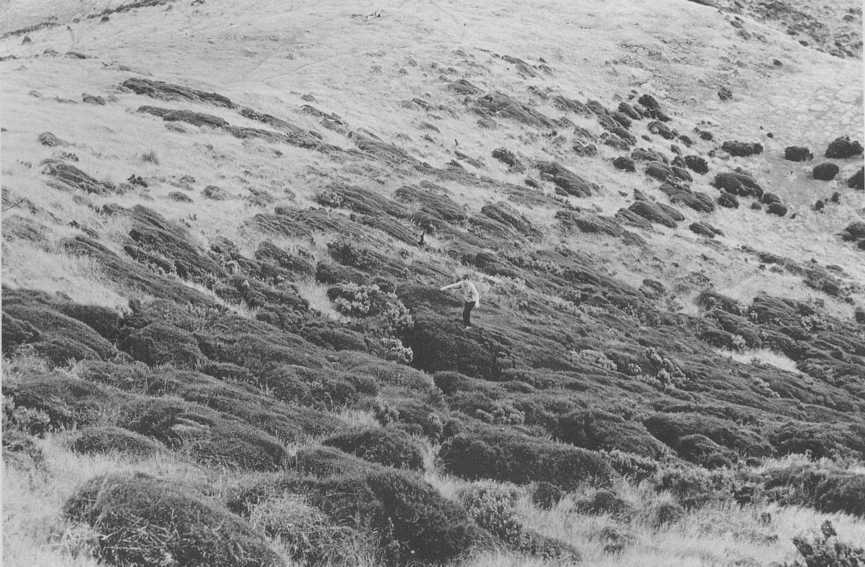
\includegraphics[width=\textwidth]{graphics/figure74shrubs.jpg}
			\caption[A remarkable windswept shrub association]{A remarkable windswept shrub association comprising a number of species of divaricate shrubs and juveniles as well as some vines.
			Note the figure standing on the surface of the shrubbery.
			Mt. Kaukau near Wellington, southern North Island.
			Photo: J. W. Dawson.}%
			\label{fig:74shrubs}
		\end{minipage}\hspace{\fgap}%
		\begin{minipage}[t]{(\textwidth-\fgap) * \real{0.297}}
			\centering
			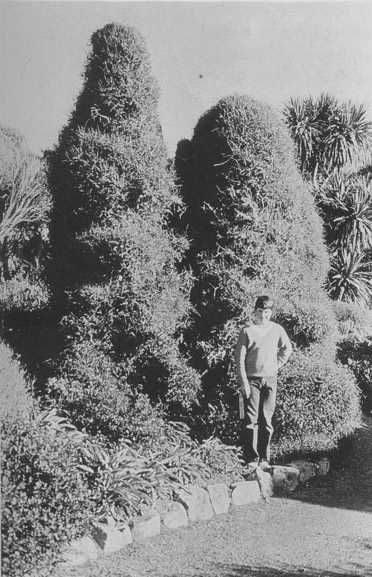
\includegraphics[width=\textwidth]{graphics/figure75pittosporum.jpg}
			\caption[Habit of heart-leaved kohuhu (\emph{Pittosporum obcordatum})]{Habit of \IDX{heart-leaved kohuhu} (\BotanicRef{Pittosporum obcordatum}[Pittosporum][obcordatum]) in cultivation at Otari Gardens, Wellington.
			Photo: J. W. Dawson.}%
			\label{fig:75pittosporum}
		\end{minipage}
	\end{minipage}
	% Outer minipage scaled to limit width.
	% Inner minipages scaled so the images have the same height.
	\begin{minipage}[t]{0.95\textwidth}
		\begin{minipage}[t]{(\textwidth-\fgap) * \real{0.354}}
			\centering
			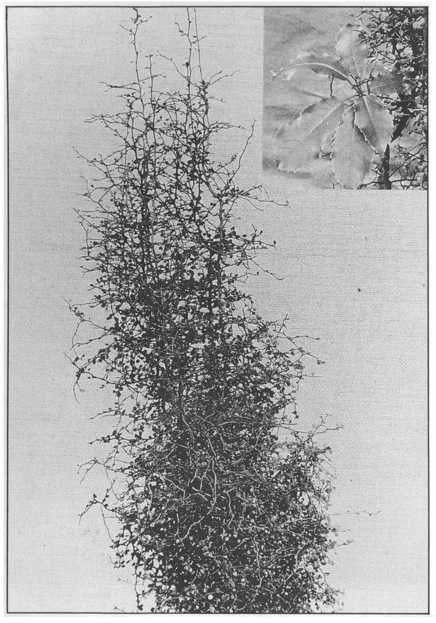
\includegraphics[width=\textwidth]{graphics/figure76pseudopanax.jpg}
			\caption[\emph{Pseudopanax anomalus}]{\BotanicRef{Pseudopanax anomalus}[Pseudopanax][anomalus].
			Although seedlings have small palmately-compound leaves, adult leaves are simple and \SIrange{1}{2}{\centi\metre} long.
			Other New Zealand species of \BotanicRef{Pseudopanax}, such as \IDX{whauwhaupaku} (\BotanicRef{Pseudopanax arboreus}[Pseudopanax][arboreus], \IDX{five-finger}) at top right and \BotanicRef{Pseudopanax laetum}[Pseudopanax][laetum], have large, palmately compound leaves with leaflets up to \SI{25}{\centi\metre} long. Photo:  J. W. Dawson.}%
			\label{fig:76pseudopanax}
		\end{minipage}\hspace{\fgap}%
		\begin{minipage}[t]{(\textwidth-\fgap) * \real{0.646}}
			\centering
			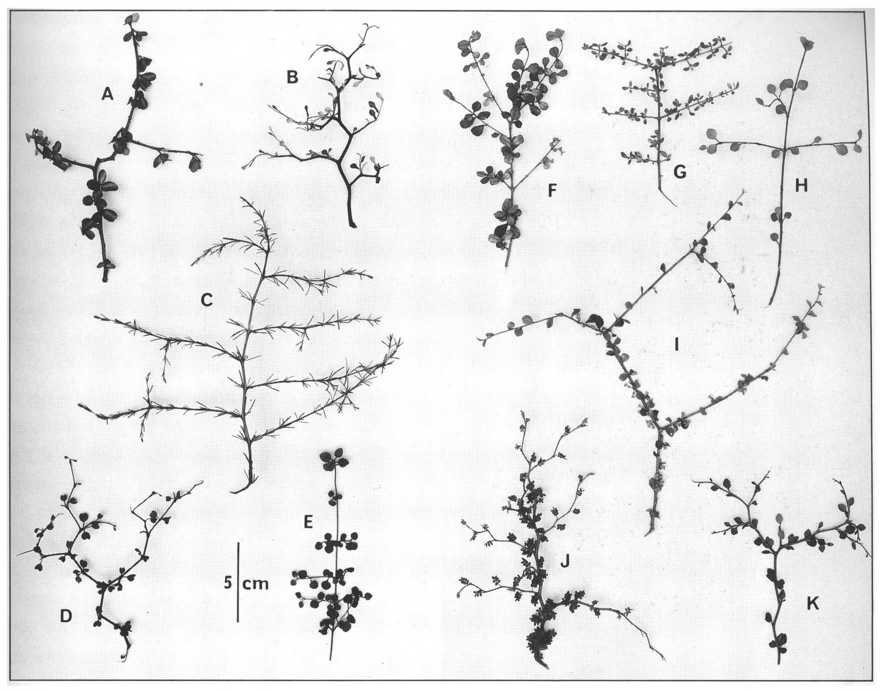
\includegraphics[width=\textwidth]{graphics/figure77twigs.jpg}
			\caption[Leafy twigs of some of the New Zealand divaricate species]{Leafy twigs of some of the New Zealand divaricate species, with one exception each from a different family:
			A, \IDX{weeping matipo} (\BotanicRef{Myrsine divaricata}[Myrsine][divaricata]).
			B, \IDX{korokio} (\BotanicRef{Corokia cotoneaster}[Corokia][cotoneaster]).
			C, \IDX{sand coprosma} (\BotanicRef{Coprosma acerosa}[Coprosma][acerosa]).
			D, \IDX{shrubby tororaro} (\BotanicRef{Muehlenbeckia astonii}[Muehlenbeckia][astonii]).
			E, \BotanicRef{Teucridium parvifolium}[Teucridium][parvifolium].
			F, \IDX{rōhutu} (\BotanicRef{Lophomyrtus obcordata}[Lophomyrtus][obcordata]).
			G, \BotanicRef{Coprosma wallii}[Coprosma][wallii].
			H, \IDX{poataniwha} (\BotanicRef{Melicope simplex}[Melicope][simplex]).
			I, \IDX{heart-leaved kohuhu} (\BotanicRef{Pittosporum obcordatum}[Pittosporum][obcordatum]).
			J, \IDX{prostrate kowhai} (\BotanicRef{Sophora prostrata}[Sophora][prostrata]).
			K, \BotanicRef{Pseudopanax anomalus}[Pseudopanax][anomalus].
			Photo:  J. E. Casey.}%
			\label{fig:77twigs}
		\end{minipage}
	\end{minipage}
\end{figure}
The result of this distinctive branching behaviour is a densely interlaced, springy, more or less balllike shrub.
Where these grow in windswept situations on hill tops or at the coast they form low hummocks which are so dense that a person can stand on them\figureref{\fullref{fig:74shrubs}}, or even jump up and down on them, without breaking through the surface.
At first acquaintance all divaricate shrubs tend to look the same, but, according to Greenwood and Atkinson,\footnote{\cite{greenwood1977evolution}} there are in New Zealand 54 species of this form (including the divaricating juveniles of some trees) belonging to 20 genera and 17 families\figureref{\fullref{fig:75pittosporum}, \fullref{fig:76pseudopanax}, \fullref{fig:77twigs}}.
A further 9 species are illustrated in Eagle's \emph{Trees and Shrubs of New Zealand}\footnote{\cite{eagle1982trees}}, but have not yet been named formally.
Nine species from an additional 6 genera (including \BotanicRef{Nothofagus}, \BotanicRef{Neomyrtus}, \BotanicRef{Lophomyrtus} and \BotanicRef{Teucridium}) and 4 families are termed semi-divaricating.
Some of these have small leaves and slender twigs but their branching angles are relatively narrow.

Some divaricate shrubs are the persistent juvenile stages of forest trees, which undergo a dramatic change in branching pattern and an equally dramatic increase in leaf size when they change to the adult state.

\begin{SCfigure}[2.0][!b]
	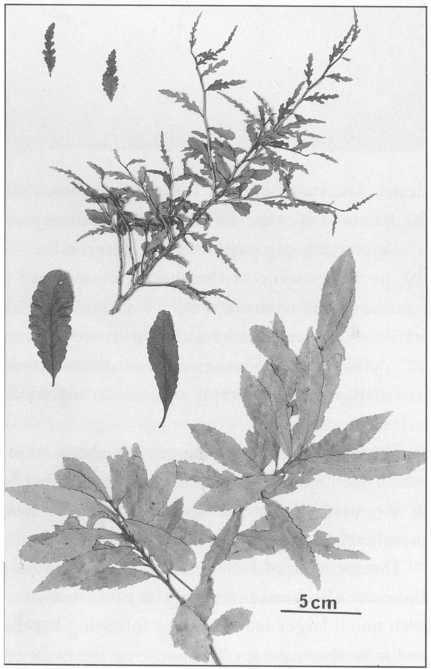
\includegraphics[width=0.5\textwidth]{graphics/figure78pokaka.jpg}
	\centering
	\caption[Pokaka]{\IDX{Pokaka}[pokaka] (\BotanicRef{Elaeocarpus hookerianus}[Elaeocarpus][hookerianus]).
	Juvenile divaricate form above, adult form below.
	Photo:  J. E. Casey.}%
	\label{fig:78pokaka}
\end{SCfigure}

Two species have divaricate juveniles with leaves which are remarkably variable from long and narrow to short and round and from deeply lobed and dissected to entire --- \IDX{pokaka} (\BotanicRef{Elaeocarpus hookerianus}[Elaeocarpus][hookerianus])\figureref{\fullref{fig:78pokaka}} and \IDX{Turner's kohuhu} (\BotanicRef{Pittosporum turneri}[Pittosporum][turneri]).
The non-divaricating vine \IDX{New Zealand jasmine} (\BotanicRef{Parsonsia heterophylla}[Parsonsia][heterophylla]) has similar juvenile leaves.
Divaricating shrubs may themselves have juvenile forms.
\IDX{Poataniwha}[poataniwha] (\BotanicRef{Melicope simplex}[Melicope][simplex]) and \BotanicRef{Pseudopanax anomalus}[Pseudopanax][anomalus] have simple adult leaves but compound juvenile leaves.
Several divaricate Pittosporums have strongly dissected or narrowly elongate juvenile leaves.
Perhaps most remarkable of all, \IDX{mountain wineberry} (\BotanicRef{Aristotelia fruticosa}[Aristotelia][fruticosa]) has a juvenile which is not divaricate, but has a similar range of leaf forms to that of \IDX{pokaka}.
Cockayne\footnote{\cite{cockayne1899enquiry}} says: `The various forms assumed by the (juvenile) leaves of \BotanicRef{Aristotelia fruticosa}[Aristotelia][fruticosa] are almost beyond belief'.

Little is yet known about the precise habits of growth of most divaricates, but it is clear that they are not uniform, for example: \begin{description}
	\item[{(a)}]in some species the interlacing tendency of the twigs is enhanced by the zig-zag pattern of the internodes;
	\item[{(b)}]in others some of the shoots remain very short and bear most of the leaves of the shrubs;
	\item[{(c)}]in those species where there is more than one bud in the leaf axils, development of some of the additional buds after a period of dormancy further complicates an already complicated branching pattern.
\end{description}

There are differences of opinion about whether divaricating shrubs which are exactly equivalent to those of New Zealand occur elsewhere in the world,\footnote{\cite{greenwood1977evolution}} but it seems that only in New Zealand are they so prevalent in both the flora and the vegetation.\footnote{A partly comparable situation exists in south-west Madagascar (\cite{koechlinj1974flore}) where in arid, but foggy, coastal sites there is an abundance of twiggy, densely interlaced, small-leaved shrubs belonging to genera from a number of different families. Some of the shrubs are spiny and some have zig-zag branching and short shoots as in New Zealand. The small-leaved shrubs of Madagascar are not related to those of New Zealand but probably derive from tree and shrub relatives with much larger leaves in the tropical rain forests.}

The majority of New Zealand divaricates belong to genera in which there are also local forest species of normal branching patterns, usually with much larger leaves.
In the following list the numbers of divaricate and non-divaricate species are given for each genus.

\begin{longtable}{ l c c c }
	\toprule
	& \emph{Divaricate} & \thead{\emph{Non-}\\ \emph{divaricate}} & \thead{\emph{Divaricate}\\ \emph{juvenile}}\\
	\midrule
	\endhead%
	\emph{Violaceae} \\
	\hspace{\fgap}Melicytus (incl. Hymenanthera) & 5\footnote{Includes some species not yet named, but illustrated in Eagle} & 8\footnote{Includes some species not yet named, but illustrated in Eagle} \\
	\emph{Polygonaceae} \\
	\hspace{\fgap}Muehlenbeckia & 1 & 4 \\
	\emph{Pittosporaceae} \\
	\hspace{\fgap}Pittosporum & 5 & 14 & 1\\
	\emph{Elaeocarpaceae} \\
	\hspace{\fgap}Elaeocarpus &  & 1 & 1\\
	\hspace{\fgap}Aristotelia & 1 & 1 \\
	\emph{Malvaceae} \\
	\hspace{\fgap}Plagianthus & 1 & & 1\\
	\hspace{\fgap}Hoheria & & 4\footnote{Includes some species not yet named, but illustrated in Eagle} & 2\\
	\emph{Escalloniaceae} \\
	\hspace{\fgap}Carpodetus &  &  & 1\\
	\emph{Leguminosae} \\
	\hspace{\fgap}Sophora & 1 & 1 & 1\\
	\emph{Moraceae} \\
	\hspace{\fgap}Streblus (Paratrophis) &  & 1 & 1\\
	\emph{Icacinaceae} \\
	\hspace{\fgap}Pennantia &  & 1 & 1\\
	\emph{Rhamnaceae} \\
	\hspace{\fgap}Discaria & 1 \\
	\emph{Rutaceae} \\
	\hspace{\fgap}Melicope & 1 & 1 \\
	\emph{Araliaceae} \\
	\hspace{\fgap}Pseudopanax & 1 & 13 \\
	\emph{Cornaceae} \\
	\hspace{\fgap}Corokia & 1 & 2 \\
	\emph{Myrsinaceae} \\
	\hspace{\fgap}Myrsine & 1 & 6 \\
	\emph{Rubiaceae} \\
	\hspace{\fgap}Coprosma & 28\footnote{Includes some species not yet named, but illustrated in Eagle} & 21 \\
	\emph{Compositae} \\
	\hspace{\fgap}Olearia & 7 & 24 \\
	\emph{Podocarpaceae} \\
	\hspace{\fgap}Prumnopitys &  & 1 & 1 \\
	\bottomrule
\end{longtable}

Greenwood and Atkinson\footnote{\cite{greenwood1977evolution}} consider that 26, or nearly half, of the divaricate species they considered are largely restricted to one vegetation type: forest (10); forest margins (3); scrubland\footnote{Greenwood and Atkinson distinguish `scrub' and `shrubland' thus: `… scrub is distinguished from forest by having most stems less than \SI{10}{\centi\metre} DBH.\@ Shrubland is distinguished from scrub by having a woody cover of less than 80 per cent'.} (5); shrubland (6); grassland and other open vegetation (2).
The other 28 species can be found in two or more vegetation types.
Some of these are remarkable in their range.
For example \BotanicRef{Coprosma rhamnoides}[Coprosma][rhamnoides] at one extreme grows in shade and shelter on open forest floors and there forms attractive shrubs with leaves which tend to be arranged in horizontal layers.
At the other extreme it may be found in the open on hill tops exposed to violent gales, where it forms or contributes to dense shrub hummocks shaped and channelled by the wind\figureref{\fullref{fig:74shrubs}}.
The fivefinger relative \BotanicRef{Pseudopanax anomalus}[Pseudopanax][anomalus] is a similar case.

\begin{SCfigure}[1.0][!b]
	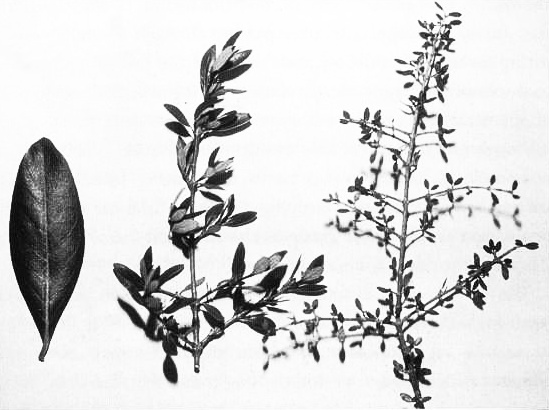
\includegraphics[width=0.66\textwidth]{graphics/figure80coprosma.jpg}
	\centering
	\caption[Hybridism in Coprosma]{Hybridism in \BotanicRef{Coprosma}.
	Left: a leaf of \IDX{karamu} (\BotanicRef{Coprosma robusta}[Coprosma][robusta]); right: twigs of \IDX{mingimingi} (\BotanicRef{Coprosma propinqua}[Coprosma][propinqua]) showing the very small leaves; centre: the natural hybrid between these two species.
	This hybrid was originally described as a species --- \BotanicRef{Coprosma cunninghamii}[Coprosma][cunninghamii].
	Allan (\cite{allan1924hybridity}) proved that it was a hybrid by artificially crossing the two species.
	Photo:  J. W. Dawson.}%
	\label{fig:80coprosma}
\end{SCfigure}

\begin{figure}[!t]
	\centering
	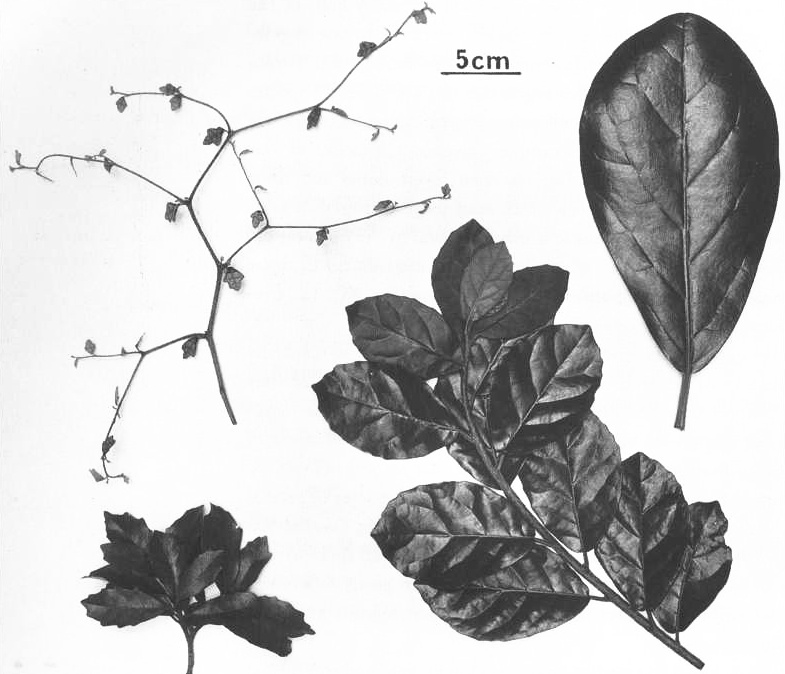
\includegraphics[width=0.75\textwidth]{graphics/figure79pennantia.jpg}
	\caption[Hybridism in Pennantia]{Hybridism in \BotanicRef{Pennantia}.
	At upper left is the small-leaved divaricate juvenile of \IDX{kaikomako} (\BotanicRef{Pennantia corymbosa}[Pennantia][corymbosa]) and at lower left a portion of the non-divaricate larger-leaved adult.
	Kaikomako ranges throughout the country and is a small tree mostly found at forest margins.
	On the right is a large, thick leaf of \IDX{Three Kings kaikomako} (\BotanicRef{Pennantia baylisiana}[Pennantia][baylisiana]).
	This, the only other species of \BotanicRef{Pennantia} in New Zealand, is restricted to the Three Kings Islands and is represented there by a single small tree.
	Like \IDX{kaikomako}, \IDX{Three Kings kaikomako} (\BotanicRef{Pennantia baylisiana}[Pennantia][baylisiana]) is dioecious and the sole tree is a female.
	It has been reproduced by cuttings and a flowering specimen is now established at Otari Plant Museum in Wellington.
	It was noticed that some berries were formed by this tree and some of the seeds in these germinated to form several identical plants now several years old, although not yet flowering.
	It seems likely that the female flowers of \IDX{Three Kings kaikomako} (\BotanicRef{Pennantia baylisiana}[Pennantia][baylisiana]) were pollinated by male plants of kaikomako in the vicinity and that the progeny are hence probably hybrids between the two species. (An alternative possibility is that the suggested hybrids are juveniles of \BotanicRef{Pennantia baylisiana}[Pennantia][baylisiana] derived from embryos without fertilisation (apomixis).) Foliage from the suggested hybrid is at the centre of the photo.
	Its leaves are dark green and shiny like those of \BotanicRef{Pennantia baylisiana}[Pennantia][baylisiana], but are much smaller and toothed like those of kaikomako.
	There is no clearly marked juvenile form in these plants.
	There are several other cases of hybrids between morphologically very different species in New Zealand --- \IDX{karamu} (\BotanicRef{Coprosma robusta}[Coprosma][robusta]) x \IDX{mingimingi} (\BotanicRef{Coprosma propinqua}[Coprosma][propinqua])\figureref{\fullref{fig:80coprosma}}, \IDX{wharangi} (\BotanicRef{Melicope ternata}[Melicope][ternata]) x \IDX{poataniwha} (\BotanicRef{Melicope simplex}[Melicope][simplex]), \IDX{korokio} (\BotanicRef{Corokia buddleioides}[Corokia][buddleioides]) x \BotanicRef{Corokia cotoneaster}[Corokia][cotoneaster] and a number of others.
	Photo:  J. E. Casey.}%
	\label{fig:79pennantia}
\end{figure}

Within the genera concerned, the `normal' species differ so markedly in appearance from the divaricates that it is difficult to believe that they are related.
Apart from the differences in branching pattern the leaves of the normal species are often hundreds of times the area of those of the divaricates.
Even more surprising is the fact that natural hybrids are not uncommon between divaricate and non-divaricate species of several genera --- \BotanicRef{Melicytus}, \BotanicRef{Aristotelia}, \BotanicRef{Sophora}, \BotanicRef{Melicope}, \BotanicRef{Tseudopanax}, \BotanicRef{Corokia}, \BotanicRef{Pennantia}, \BotanicRef{Myrsine}, \BotanicRef{Coprosma}\footnote{\cite{allan1924hybridity}}\figureref{\fullref{fig:80coprosma}, \fullref{fig:79pennantia}} (3 pairs of species) and \BotanicRef{Olearia}.
In some cases the first generation hybrids are partly fertile and give rise to bewildering arrays of second generation hybrids known as `hybrid swarms'.

It is generally believed that the divaricates are derived and specialised forms and the fact that a number of them are able to hybridise with large-leaved relatives might indicate that this distinctive growth habit evolved in relatively recent geological times.

We now come to the problem of how and why divaricate plants became such a conspicuous feature of the New Zealand flora.
If there were only one species of this form it might be dismissed as a chance aberration, but as there are many, and these are mostly unrelated to one another, some special environmental factor or combination of factors selecting for the habit is indicated.
A contrary view is that of Went,\footnote{\cite{went1971parallel}} who suggests a virus-like transmission of chromosome segments, bearing divarication inducing factors, from species to species, genus to genus and family to family.
Because of the difficulty of envisaging a mechanism for such transfers this idea has not received much support, although it does not seem so outlandish in these days of genetic engineering as it would have done some years ago.

\section{Climatic Theories}

However, most theories about divaricating shrubs regard them as an example of parallel evolution in response to some environmental factor, but there is little agreement yet on what that factor is.
The first to speculate late last century was Diels,\footnote{\cite{diels1897vegetations}} who as a young man wrote a remarkable thesis on New Zealand vegetation even though at that stage he had not seen it.
He based his account on herbarium and living plants available to him in Berlin, earlier publications and information from correspondents including Cockayne.
Diels concluded that the divaricate habit was an adaptation to drought and suggested that shrubs with this form had evolved from forest ancestors at a time when the South Island axial ranges were higher than they are now and the rain shadow effect to the east of them, accentuated by drying winds, was much more extreme.
Diels also suggested that coldness during glacials was a contributing factor in the evolution of this growth form, and Rattenbury\footnote{\cite{rattenbury1962cyclic}} later suggested that the influence of coldness could have been indirect by inducing physiological drought of the root systems.
Cockayne\footnote{\cite{cockayne1912observations}} accepted and extended Diels' interpretation, paying particular attention to trees with divaricating juveniles.
He saw these as being ultimately derived from pre-ice age tree ancestors which completely lacked divaricate branching at any stage.
During the cold and dry conditions in the east during glacials divaricating shrubs evolved from the trees and with the return of warmer, moister conditions some of these regained their tree form, although only after passing through a small-leaved, divaricating juvenile phase.
Cockayne regarded the last growth pattern as an example of `ontogeny recapitulating phylogeny', that is the persistance of ancestral traits in the embryonic or, in this case, juvenile phase of a life cycle.
In support of this evolutionary sequence he noted that \IDX{manatu} (\BotanicRef{Plagianthus regius}[Plagianthus][regius], \IDX{ribbonwood}) has a divaricating juvenile on the main islands but not on the outlying Chatham Islands.
He regarded the population on the latter group as the ancestral form, which survived in the milder, oceanic climate of a small island.

Wardle\footnote{\cite{wardle1963evolution}} took a different view of trees with divaricating juveniles.
Noting that divaricates generally are conspicuous in `dryish' eastern forests, he suggested that divaricate juveniles might relate to existing climates which tend to periodic drought and that the changeover to the larger-leaved adult form takes place once a deep, efficient root system has developed.
At times of greater aridity, perhaps during glacials, some divaricate juveniles would become `fixed' flowering and fruiting divari-cate shrubs.
Thus according to Cockayne the sequence would have been: non-divaricating tree --- divaricating shrub --- tree with divaricating juvenile; and according to Wardle: non-divaricating tree --- tree with divaricating juvenile --- divaricating shrub.

More recently, Wardle's hypothesis concerning microphyllous juveniles has been applied on Reunion and Mauritius Islands in the Indian Ocean where microphyllous, although not divaricating, juveniles are unusually common on the drier sides of the islands.\footnote{\cite{friedmann1976observations}}

With regard to \BotanicRef{Sophora}, Cockayne held a view in conflict with his own theory but in accord with that of Wardle: the divaricate shrub \IDX{prostrate kowhai} (\BotanicRef{Sophora prostrata}[Sophora][prostrata]) is interpreted as a flowering and fruiting fixed juvenile of \IDX{small-leaved kowhai} (\BotanicRef{Sophora microphylla}[Sophora][microphylla]).
Godley questions this view,\footnote{\cite{godley1979leonard}} pointing out that the leaves and stems of \IDX{prostrate kowhai} (\BotanicRef{Sophora prostrata}[Sophora][prostrata]) and the divaricate juvenile of \IDX{small-leaved kowhai} (\BotanicRef{Sophora microphylla}[Sophora][microphylla]) are quite dissimilar, as are the flowers and seed pods of the two species.
He proposes an interesting and quite different explanation --- the extremely variable \IDX{small-leaved kowhai} (\BotanicRef{Sophora microphylla}[Sophora][microphylla]) (with everything from non-divaricate to strongly divaricate juveniles depending on locality) may derive from an ancient hybridisation between the non-divaricate and relatively largeleaved small tree \IDX{large-leaved kowhai} (\BotanicRef{Sophora tetraptera}[Sophora][tetraptera]) and the dwarf divaricate shrub \IDX{prostrate kowhai} (\BotanicRef{Sophora prostrata}[Sophora][prostrata]).
He further suggests that all trees with divaricate juveniles may have originated in a similar way.

McGlone and Webb,\footnote{\cite{mcglone1981selective}} in response to the `moa theory', which we will consider later, reaffirmed and refined the climatic explanation of the divaricating habit.
They believe:

\begin{quote}
	that the divaricating habit is an adaptation which enables the plant to resist damage from wind, frost and desiccation, while retaining enough flexibility to exploit a wide range of habitats.
\end{quote}

They relate this growth habit to what they regard as New Zealand's distinctive climate:

\begin{quote}
	as a consequence of its position in the mid-latitudes and its isolation in a large area of ocean, New Zealand has a mild, generally humid, windy climate.
	However, it is also a very variable climate and the continental pattern of a cold winter and a consistently warm summer does not apply here.
\end{quote}

They point out that in many forest areas in New Zealand, night frosts may occur at any time of the year, often to be followed by quite warm days.
Also in areas to the east of the mountain ranges, dry often very warm föhn winds may be frequent in spring and summer and are sometimes followed by cool or even frosty weather especially inland.
In such circumstances deciduousness would seem an inappropriate adaptation, but McGlone and Webb believe that the mostly evergreen\footnote{\IDX{Shrubby tororaro}[shrubby tororaro] (\BotanicRef{Muehlenbeckia astonii}[Muehlenbeckia][astonii]) and a few divaricate species of Olearia are deciduous.} smallleaved divaricating shrub is well suited to survive the inclement and to take advantage of the favourable spells of weather.
They see the balllike divaricating shrub, with its internal as well as external twigs, growing points and leaves, serving as a wind screen, frost screen and heat trap.
With regard to wind they see three benefits for the internal leaves, which outweigh the disadvantage of their being partially shaded: the drying effect of the wind is reduced; abrasion by wind-borne particles is reduced; and the tendency of the interlaced mass of twigs to move as a whole means that twigs and leaves are less likely to hit each other and become damaged.
With frost they have observed in a number of divaricating species that `even in severe frosts in which exposed leaves are frozen the interior leaves of the shrubs are unaffected'.
Finally, concerning the heat trap idea, they say:

\begin{quote}
	besides possibly acting as a frost screen, the protective network of branches may, on cold, but sunny days, act as a heat trap, raising the temperature of the air mass inside the shrub, and this may permit higher rates of photosynthesis.
\end{quote}

With divaricate juveniles McGlone and Webb agree with Wardle that the changeover to the adult form may follow the development of a deep root system, but also suggest that the changeover may take place once a height above ground frost level is attained.

They suggest that the genera in New Zealand which have some divaricating species probably originated under at least subtropical conditions and had the opportunity to evolve cold-tolerant forms because New Zealand's isolation and lack of mountains during the Tertiary largely precluded the establishment of genera which had evolved in colder climates:

\begin{quote}
	we believe that the divaricating plant habit was one of the responses of this essentially subtropical flora to the onset of glacial climates.
\end{quote}

Indeed, evidence of trends in branching patterns and leaf sizes in tropical and subtropical forest genera in relation to decreasing temperature does indicate that the divaricating habit might represent the end point of such trends.
In places in the world such as coastal Brazil,\footnote{\cite{cain1956applications}} where rain forest extends from the equator to subtropical latitudes, a correlation has been observed between decreasing temperatures with increasing distance from the equator and a replacement of big-leaved, sparsely branched species with progressively smaller-leaved and more freely branched species.
New Zealand's isolation when climates became colder would have enabled such a trend to continue to its ultimate extreme.

\section{Moa Theory}

We come now to the `moa\footnote{Moas were flightless birds, some species of which were larger than emus or ostriches. They became extinct a few centuries before the arrival of Europeans.} theory' elaborated by Greenwood and Atkinson,\footnote{\cite{greenwood1977evolution}} which has found favour with some but disbelief from others.
Some of the negative reactions, I think, stem from the fact that the moas are extinct.
The `moa theory' has a science fiction ring to it, just as would a `dodo theory' or, to extend into myth, a `dragon theory'.
At our present state of knowledge, however, the moa theory merits serious consideration along with the climatic theories.

Essentially, Greenwood and Atkinson propose that the divaricating shrub habit is probably unique to New Zealand and results from an environmental factor that was also unique to New Zealand, namely the moas.
Species of similar appearance to divaricating shrubs elsewhere in the world either have relatively large leaves and/or are spiny.
Spininess of shrubs is considered to be a defence against the browsing of softnosed mammals, but it would be ineffective against large, browsing birds with their hard beaks.
With the exception of \IDX{matagouri} (\BotanicRef{Discaria toumatou}[Discaria][toumatou]) New Zealand divaricates are not spiny, although there is a tendency that way with some reduced shrubs in exposed habitats.
\IDX{Matagouri}[matagouri] has spiny relatives in Australia and South America so probably evolved its spininess outside New Zealand.

Greenwood and Atkinson considered the essential features of divaricating shrubs to be: interlaced branching; small leaf size; stem toughness; and leaves which are smaller on outer than on inner branches.
In their original publication they assumed that moas could not bite with a cutting action, but clamped, pulled and broke off portions of foliage This would have made it difficult for them to browse on divaricates as the twigs are wiry and difficult to pull off and, when broken, difficult to disentangle.
It was further suggested that where the outermost twigs had very reduced leaves and a dead appearance they would be rejected as unpalatable.
With regard to trees with divaricating juveniles, they suggest that the change to adult branching and foliage took place above the reach of moas.

Later work showed that the assumption about moa eating habits was incorrect.
Burrows\footnote{\cite{burrows1980moas}} examined the plant material contained in fossilised moa gizzards and found that it mostly `consisted of twigs, commonly \SIrange{1.5}{6.0}{\milli\metre} thick and \SIrange{10}{30}{\milli\metre} long.
Some of these twigs are of \IDX{twiggy tree daisy} (\BotanicRef{Olearia virgata}[Olearia][virgata]) and \IDX{manatu} (\BotanicRef{Plagianthus regius}[Plagianthus][regius]) (both divaricating species) and much material appears to have come from \BotanicRef{Coprosma}, a genus which contains a large number of divaricating species.
Most of the twigs were cleanly cut, probably by the shearing action of the moa beak, rather than broken'.

Greenwood and Atkinson\footnote{\cite{atkinson1980divaricating}} and Lowry\footnote{\cite{lowry1980evolution}} suggested that although the divaricate habit may not have prevented moa browsing, the many growing points separated by the wide branching angles would have enabled plants of this form to survive and quickly recover from browsing.

Greenwood and Atkinson note that divaricates are most abundant on fertile soils such as those of river flats and suggest that this is because plants on such sites would be more nutritious and therefore favoured by moas.
On the other hand they point out that there are few divaricates on outlying islands not reached by moas and none on cliffs or as epiphytes on branches: `moas would have experienced difficulty in browsing either on cliffs or up trees'!

In opposition to this view, McGlone and Webb\footnote{\cite{mcglone1981selective}} suggest that the prevalence of divaricates on river flats and similar places derives from the fact that such sites are particularly frosty.
They also ask why divaricates, if they were maintained on river flats by browsing, have not been replaced in the centuries since moa extinction by faster growing, larger-leaved shrubs and trees.

To throw yet another hat into the ring, river flats are also subjected to floods from time to time, so perhaps the divaricate habit is flood-resistant and in trees with divaricate juveniles the change to the adult state takes place above flood level? It is perhaps relevant here that McGlone and Webb believe that river beds, dunes and wind-induced scrub were probably the only places in the lowlands during the warmest phases of the interglacials, which could serve as refugia for divaricates.
The `flood' hypothesis undoubtedly raises a number of questions, such as why there are no divaricates within the flood zone of river cliffs, but it is not alone in this respect.
Perhaps divaricate plants are tolerant of a number of environmental factors rather than just one.

The one thing that is clear in all of this is that the divaricating shrub story has not yet been fully told and that we need to know much more about the morphological, physiological and ecological details of the plants concerned.

Finally, not all small leaved shrubs in New Zealand are of divaricate form.
The large genus \BotanicRef{Hebe} has many scale-leaved `whipcord' species, mostly found at higher altitudes, which are probably derived forms, as are the many needle-leaved species of \BotanicRef{Dracophyllum} and some small-leaved but not divaricating species of \BotanicRef{Olearia}, \BotanicRef{Coprosma} and other genera.
We need to keep these in mind when theorising about shrubs which are divaricating as well as small-leaved.
